\section{VeriFast}

Im Rahmen dieser Seminararbeit werden wir uns hauptsächlich mit dem Verifikationswerkzeug \emph{VeriFast} auseinandersetzen, dass in Form eines Prototypen an der KU Leuven ins Leben gerufen wurde und aktiv weiterentwickelt wird. VeriFast erlaubt die Verifikation von \emph{single-} und \emph{multithreaded} C und Java Programmen, welche mit zusätzlichen Annotationen für die Verifikation bestimmter Korrektheitseigenschaften ausgestattet sind. Die Annotationen stehen innerhalb von Kommentaren, wodurch der verifizierte C Code ohne zusätzliche Änderungen kompiliert werden kann. Während der Ausführung von VeriFast wird das Programm auf illegale Speicherzugriffe, beispielsweise durch Dereferenzierung von Null-Pointern oder durch Zugriff auf Speicherzellen außerhalb der Grenzen eines Arrays, sowie Fehler aufgrund nebenläufiger Ausführung geprüft. Darüber hinaus verifiziert VeriFast die annotierten Methoden-Kontrakte - d.h. es wird versucht zu zeigen, dass sich die Nachbedingung aus der Vorbedingung und der symbolischen Ausführung des Methodenrumpfs ergibt. Diesbezüglich wird im Back-End der SMT Solver \emph{Z3} von Microsoft verwendet. \cite{Jacobs2010}

\begin{figure}[!hbt]
	\centering
	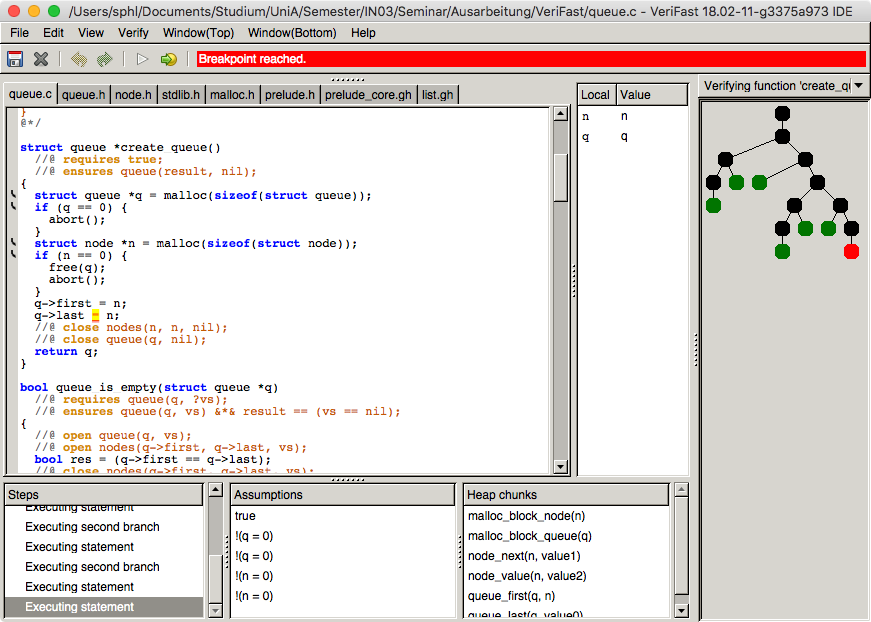
\includegraphics[width=0.8\linewidth]{verifast}
	\caption{VeriFast IDE}
	\label{fig:vfide}
\end{figure}

\noindent
Über die VeriFast IDE (siehe \vref{fig:vfide}) können Quellcodedateien editiert und Programme schrittweise/in einem Durchlauf verifiziert werden. Im Falle eines Fehlers werden diese innerhalb des Editors lokalisiert und anhand einer Statusmeldung dem Benutzer mitgeteilt. Wurde die Verifikation erfolgreich durchlaufen, so können abhängig von der ausgewählten Funktion die getesteten Pfade in Form eines Ausführungsbaums angezeigt werden. Zudem ermöglicht VeriFast über das Anklicken eines Blattknotens die Analyse einzelner Pfade. Die \emph{steps}-Auswahl listet hierbei die ausgeführten Schritte eines Pfades auf und erlaubt Sprünge zu vorherigen bzw. nachfolgenden Zuständen. Nebenan befinden sich die logischen Annahmen (\emph{assumptions} bzw. \emph{path constraints}), die sich aus den Annotationen und dem ausgeführten C Code ergeben. Eine Besonderheit der IDE ist die Anzeige der \emph{heap chunks}, welche abhängig vom Ausführungsschritt den symbolischen Zustand des Heap-Speichers darstellen. Darüber befindet sich eine weitere Auswahl, welche einen Überblick über die Zuordnung der lokalen Variablen auf deren symbolischen Werte gibt.

\subsection{Sprachkonstrukte}

In diesem Abschnitt werden einige (Sprach-)Konzepte vorgestellt die VeriFast für die Programmverifikation bereitstellt. Dabei werden vorzugsweise die Konzepte behandelt, welche für das Verständnis des Beispiels in \cref{subsec:queue} relevant sind. Weiterführende Konzepte und Beispiele können in \cite{Jacobs2017} nachgelesen werden.

\subsubsection{Induktive Datentypen}
\label{subsec:adt}

Ein wichtiges Hilfsmittel um die Korrektheit von Programme nachzuweisen, besteht in der Spezifikation von abstrakten Datentypen (ADT). Diese ermöglichen es, Eigenschaften und Operationen eines Datentyps auf einem höheren Abstraktionsniveau, d.h. unabhängig der konkreten Implementierung auf einem Computer, zu betrachten. Daraus resultierend können ADTs in der Programmverifikation als Repräsentanten für die Inhalte konkrete Datenstrukturen, wie beispielsweise Array oder einfach/doppelt verkettete Listen, eingesetzt werden. \cite[S. 265]{Saake2014}

VeriFast unterstützt den Einsatz von induktiven Datentypen, deren Instanzen über die Konkatenation von Konstruktoren (Konstruktorterm) gebildet werden. Die Spezifikation einer abstrakten Liste sieht dabei wie folgt aus.

\begin{lstlisting}
inductive list<t> = nil | cons(t, list<t>);
\end{lstlisting}

\noindent
In diesem Beispiel wurde eine generische Liste mit den Konstruktoren \texttt{nil} für die leere Liste und \texttt{cons} für die zusammengesetzte Liste, mit Kopfelement \texttt{t} und Restliste \texttt{list<t>}, definiert. Analog zu den meisten Programmiersprachen spezifiziert \texttt{<t>} den generischen Datentyp, wodurch Listen über \texttt{int}, \texttt{char}, \texttt{bool} etc. konstruiert werden können. So entspricht der Konstruktorterm \texttt{cons('a', cons('b', cons('c', nil)))} einer Liste mit der Zeichenfolge \texttt{<'a', 'b', 'c'>}.

\subsubsection{Fixpunkt Funktionen}

Neben den induktiven ADTs unterstützt VeriFast die Spezifikation von Fix\-punkt-Funktionen, wodurch spezifische Operation auf induktive Datentypen ausgeführt werden können. Diese werden mit \texttt{fixpoint} eingeleitet und erhalten über die Parameterliste einen oder mehrere ADTs. Im Funktionsrumpf kann entweder direkt eine \texttt{return}-Anweisung, welche die berechnete Eigenschaft an den Aufrufer zurückgibt, oder eine \texttt{switch}-Anweisung stehen. Letztere führt eine Fallunterscheidung bezüglich aller Konstruktoren von genau einem induktiven Argument (Fixpunkt) aus. Zudem prüft VeriFast jede Funktion auf Terminierung - d.h. im Falle eines rekursiven Aufrufs muss der neue Fixpunkt ein Teilterm des alten Konstruktorterms sein. \cite{Jacobs2010}

Ausgehend von der induktiven Liste in \cref{subsec:adt}, definieren wir die beiden Funktionen \texttt{head} und \texttt{tail}, welche das Kopfelement bzw. die Restliste des Fixpunkts \texttt{xs} zurückliefern.

\begin{lstlisting}
fixpoint t head<t>(list<t> xs) {
  switch (xs) {
    case nil: return default_value<t>;
    case cons(x, xs0): return x;
  }
}

fixpoint list<t> tail<t>(list<t> xs) {
  switch (xs) {
    case nil: return nil;
    case cons(x, xs0): return xs0;
  }
}
\end{lstlisting}

\noindent
Für den Konstruktor \texttt{cons(t, list<t>)} bindet VeriFast die entsprechenden Werte an die Variablen \texttt{x} und \texttt{xs0}, welche im Anschluss beliebig weiterverwendet werden können. Ein Sonderfall in diesem Beispiel ist der Konstruktor \texttt{nil} in \texttt{head}. Hierbei wird ein Defaultwert zurückgegeben, der je nach Anforderung und Datentyp unterschiedliche Werte annehmen kann.

Eine weitere bekannte Funktion auf Container-Datentypen ist \texttt{length}, welche in diesem Beispiel die Länge einer Liste rekursiv berechnet. Wurde ein Term ungleich \texttt{nil} übergeben, so wird dieser sukzessive abgebaut und zugleich die Länge um den Wert 1 erhöht. Der letzte Aufruf endet immer im \texttt{nil}-Konstruktor, welcher folgerichtig den die Länge 0 zurückgibt und damit die Berechnung abschließt.\footnote{\texttt{head}, \texttt{tail}, \texttt{length} und weitere Fixpunkt-Operationen auf \texttt{list<t>} sind Bestandteil der VeriFast-Bibliothek.}

\begin{lstlisting}
fixpoint int length<t>(list<t> xs) {
  switch (xs) {
    case nil: return 0;
    case cons(x, xs0): return 1 + length(xs0);
  }
}
\end{lstlisting}

\subsubsection{malloc\_block Einheiten}

Charakteristisch für C ist die dynamische Speicherverwaltung mittels \texttt{malloc} und \texttt{free}. Dadurch kann eine festgelegte Anzahl an Bytes angefordert und falls erfolgreich vom Betriebssystem alloziert, über einen Zeigen auf den Heap-Speicher angesprochen werden. Da C über keine automatische \emph{Garbage Collection} (GC) verfügt, steht der Programmierer in der Pflicht den Speicherbereich manuell mit Hilfe von \texttt{free} zu räumen, falls dieser nicht mehr benötigt wird.

Den Zustand des Heap-Speichers gilt es auch bei der Verifikation von Programmen zu berücksichtigen. Hierbei legt VeriFast sogenannte \emph{chunks} auf dem symbolischen Heap ab, wann immer eine Datenstruktur während der symbolischen Ausführung alloziert wird. Instanzen die über \texttt{malloc} erzeugt wurden, erhalten dabei zusätzlich einen \texttt{malloc\_block} chunk. Über diesen Mechanismus kann vor der Freigabe überprüft werden, ob die zu löschende Instanz über einen gültigen \texttt{malloc\_block} Eintrag verfügt. \cite{Jacobs2008,Jacobs2010}

Das nachfolgende Listing zeigt die beiden C-Strukturen \texttt{node} und \texttt{queue}. Erstere stellt einen Knoten in einer einfach verketteten Liste dar, welche neben einer Character Variablen einen Zeiger auf das nächste Listenelement enthält. \texttt{queue} verfügt über zwei Zeiger die jeweils auf das erste bzw. letzte Element einer Liste/Warteschlange zeigen.

\vspace{-10pt}
{\noindent
\begin{minipage}[t]{.45\textwidth}
\begin{lstlisting}
struct node {
  struct node *next;
  char value;
};
\end{lstlisting}
\end{minipage}
\hfill
\begin{minipage}[t]{.45\textwidth}
\begin{lstlisting}
struct queue {
  struct node *first;
  struct node *last;
};
\end{lstlisting}
\end{minipage}
}

\noindent
Die Funktion \texttt{create\_queue}\footnote{\texttt{requires}, \texttt{ensures} und \texttt{close} werden erst in den darauffolgenden Abschnitten erklärt und können in diesem Beispiel übersprungen werden.} alloziert Heap-Speicher für eine neue Queue und weist den Variablen \texttt{first} und \texttt{last} initial den gleichen Knoten zu. Abschließend wird der Zeiger auf die Queue an den Aufrufer zurückgegeben. 

\begin{lstlisting}[label=lst:create_queue]
struct queue *create_queue()
  //@ requires true;
  //@ ensures queue(result, nil);
{
  struct queue *q = malloc(sizeof(struct queue));
  if (q == 0) { abort(); }
  struct node *n = malloc(sizeof(struct node));
  if (n == 0) { abort(); }
  q->first = n;
  q->last = n;
  //@ close nodes(n, n, nil);
  //@ close queue(q, nil);
  return q;
}
\end{lstlisting}

\noindent
\cref{tab:heap-chunks} zeigt einen Ausschnitt des symbolischen Heap-Speichers während der Ausführung von \texttt{create\_queue}. Dabei stehen die symbolischen Werte \texttt{value1} und \texttt{value2} für beliebige Werte, da keine konkrete Zuweisung für die Variablen \texttt{next} und \texttt{value} des Knotens \texttt{n} vorgenommen wurde.

{\setlength\extrarowheight{5pt} % Vergroeßert den Zeilenabstand
\begin{table}[hbt!]
%	\centering
	\begin{tabularx}{\textwidth}{|p{4.5cm}|X|}
		\hline
		\rowcolor{LightGrey1}
		%-----------------------------------------------------------------------------------------------------
		\textbf{Chunk}                   & \textbf{Beschreibung}                                     \\ \hline
		%-----------------------------------------------------------------------------------------------------
		\texttt{malloc\_block\_node(n)}  & Dynamisch allozierte Instanz \texttt{n}                   \\ \hline
		\texttt{malloc\_block\_queue(q)} & Dynamisch allozierte Instanz \texttt{q}                   \\ \hline
		\texttt{n->next |-> value1}      & Feld \texttt{next} hat symbolischen Wert \texttt{value1}  \\ \hline
		\texttt{n->value |-> value2}     & Feld \texttt{value} hat symbolischen Wert \texttt{value2} \\ \hline
		\texttt{q->first |-> n}          & Feld \texttt{first} zeigt auf Instanz \texttt{n}          \\ \hline
		\texttt{q->last |-> n}           & Feld \texttt{last} zeigt auf Instanz \texttt{n}           \\ \hline
		%-----------------------------------------------------------------------------------------------------
	\end{tabularx}
	\caption{Heap chunks}
	\label{tab:heap-chunks}
\end{table}
}

\subsubsection{Kontrakte}

Kontrakte beschreiben einen Vertrag zwischen dem Aufrufer einer Methode und der Methode selbst. Dabei besitzt jede Methodendeklaration eine Vor- und Nachbedingung, welche angeben, dass wenn die Vorbedingung (vom Aufrufer) erfüllt wird, die Nachbedingung zugesichert werden kann. Zuvor gilt es allerdings für jeden Kontrakt zu zeigen, dass die Nachbedingung aus der Vorbedienung und der symbolischen Ausführung des Methodenrumpfs folgt.

Kontrakte werden auch von VeriFast eingelesen um die Korrektheit von C-Funktionen nachzuweisen. Für die Vor- und Nachbedingung stehen die Annotationen \texttt{requires} und \texttt{ensures} zur Verfügung, deren Bedingung in Form einer \emph{Assertion} definiert wird, die sich wiederum aus Heap chunks und/oder booleschen Ausdrücken zusammensetzt. Diese können innerhalb einer Assertion mittels \emph{Separation Conjunction} $(\&{*}\&)$, aus der \emph{Separation Logic}, kombiniert werden. Allgemein beschreibt Separation Logic eine Erweiterung der \emph{Hoare Logic}, welche Schlussfolgerungen über geteilte, änderbare Datenstrukturen, wie z.B. der Heap in Java und C, erlaubt. Die Konjunktion $C_{1} \; \&{*}\& \; C_{2}$ beschreibt dabei, dass $C_{1}$ und $C_{2}$ auf disjunkten Speicherbereichen gelten und somit Änderungen keinen Einfluss bzw. Nebeneffekte auf andere Bereiche haben. \cite{Reynolds2002}

Um zu zeigen, dass die Vorbedingung bei einem Methodenaufruf erfüllt wird, versucht VeriFast die in \texttt{requires} hinterlegte Assertion zu \emph{konsumieren} - d.h. die enthaltenen Chunks und logischen Ausdrücke werden vom symbolischen Heap bzw. aus der Liste der Assumptions entfernt. Ist dies nicht möglich, da bspw. ein zu konsumierender Chunk auf dem Heap nicht vorhanden ist, so schlägt die Verifikation fehl. Konnte hingegen die Vorbedingung gezeigt werden, so \emph{produziert} VeriFast neue Einträge für die Assertion in \texttt{ensures}, die im weiteren Verlauf der Verifikation zur Verfügung stehen. Dieser Vorgang hat den Vorteil, dass bei einem Aufruf nicht der komplette Methodenrumpf durchlaufen werden muss, sondern VeriFast lediglich die spezifizierten Assertions konsumiert/produziert. \cite{Jacobs2017}

\subsubsection{Prädikate}

Prädikate können dazu eingesetzt werden, Aussagen, die wiederkehrend in unterschiedlichen Methodenkontrakten Verwendung finden, zu kapseln. Über den \texttt{close}-Befehl werden diese durch ein passendes Prädikat gebündelt, wobei die vorherige Assertion durch das entsprechende Prädikat auf dem Heap ersetzt wird. Die entgegengesetzte Wirkung erzielt \texttt{open}, dass ein Prädikat in dessen Bestandteile (Aussagen) zerlegt. \cite{Jacobs2008,Jacobs2017}

\begin{figure}[hbt!]
%	\centering
	\begin{minipage}{.45\textwidth}
%		\centering
		\begin{tikzpicture}[scale=5.5]
	\draw [thick, white] (0.05,0.65) rectangle (1.0,0.0);
	\draw [thick, black, pattern color=LightGrey3, pattern=north east lines] (0.35,0.05) rectangle (0.95,0.45);
	% First row
	\draw [fill=LightGrey1] (0.1,0.1) rectangle (0.3,0.2) node[pos=.5] {$C_{7}$};
	\draw [fill=LightGrey1] (0.1,0.3) rectangle (0.3,0.4) node[pos=.5] {$C_{4}$};
	\draw [fill=LightGrey1] (0.1,0.5) rectangle (0.3,0.6) node[pos=.5] {$C_{1}$};
	% Second row
	\draw [fill=LightGrey1] (0.4,0.1) rectangle (0.6,0.2) node[pos=.5] {$C_{8}$};
	\draw [fill=LightGrey1] (0.4,0.3) rectangle (0.6,0.4) node[pos=.5] {$C_{5}$};
	\draw [fill=LightGrey1] (0.4,0.5) rectangle (0.6,0.6) node[pos=.5] {$C_{2}$};
	% Third row
	\draw [fill=LightGrey1] (0.7,0.1) rectangle (0.9,0.2) node[pos=.5] {$C_{9}$};
	\draw [fill=LightGrey1] (0.7,0.3) rectangle (0.9,0.4) node[pos=.5] {$C_{6}$};
	\draw [fill=LightGrey1] (0.7,0.5) rectangle (0.9,0.6) node[pos=.5] {$C_{3}$};
\end{tikzpicture}
		\captionof{figure}{Prädikat \texttt{nodes}}
		\label{fig:nodes}
	\end{minipage}
	\hfill
	\begin{minipage}{.45\textwidth}
%		\centering
		\begin{tikzpicture}[scale=5.5]
	\draw [thick, black, pattern color=LightGrey2, pattern=crosshatch dots] (0.05,0.5) rectangle (1.0,0.0);
	\draw [thick, black, preaction={fill, white},pattern color=LightGrey3, pattern=north east lines] (0.35,0.05) rectangle (0.95,0.45);
	% First row
	\draw [fill=LightGrey1] (0.1,0.1) rectangle (0.3,0.2) node[pos=.5] {$C_{2}$};
	\draw [fill=LightGrey1] (0.1,0.3) rectangle (0.3,0.4) node[pos=.5] {$C_{1}$};
	% Second row
	\draw [fill=LightGrey1] (0.4,0.1) rectangle (0.6,0.2) node[pos=.5] {$C_{4}$};
	\draw [fill=LightGrey1] (0.4,0.3) rectangle (0.6,0.4) node[pos=.5] {$C_{3}$};
	% Third row
	\draw [fill=LightGrey1] (0.7,0.1) rectangle (0.9,0.2) node[pos=.5] {$C_{6}$};
	\draw [fill=LightGrey1] (0.7,0.3) rectangle (0.9,0.4) node[pos=.5] {$C_{5}$};
\end{tikzpicture}
		\captionof{figure}{Prädikat \texttt{queue}}
		\label{fig:queue}
	\end{minipage}
\end{figure}

\noindent
\cref{fig:nodes} veranschaulicht die erste \texttt{close}-Anweisung in \texttt{create\_queue} aus Listing \ref{lst:create_queue}. In dieser Abstraktion wird ein Teil der generierten Chunks ($C_{3},\ldots,C_{6}$) durch das Prädikat \texttt{nodes} gekapselt, dass wiederum in \texttt{queue} enthalten ist (vgl. \cref{fig:queue}). Die konkrete Implementierung der beiden Prädikate sieht somit wie folgt aus.

\vspace{-10pt}
{\noindent
\begin{minipage}[t]{.45\textwidth}
\begin{lstlisting}
predicate nodes(
    struct node *first,
    struct node *last,
    list<char> vs) =
  first == last ?
    vs == nil
  :
    first->next |-> ?next &*&
    first->value |-> ?val &*&
    malloc_block_node(first) &*&
    nodes(next, last, ?vs0) &*&
    vs == cons(val, vs0);
\end{lstlisting}
\end{minipage}
\hfill
\begin{minipage}[t]{.45\textwidth}
\begin{lstlisting}
predicate queue(
    struct queue *q,
    list<char> vs) =
  q->first |-> ?first &*&
  q->last |-> ?last &*&
  malloc_block_queue(q) &*&
  nodes(first, last, vs) &*&
  last->next |-> _ &*&
  last->value |-> _ &*&
  malloc_block_node(last);
\end{lstlisting}
\end{minipage}
}

\noindent
Innerhalb der oberen Listings werde neue Variablen mittels \texttt{?var} (Fragezeichen) eingeführt. Der symbolische Wert wird dabei an den Variablennamen gebunden, um somit explizite Aussagen über Werte machen zu können. Anders verhält es sich mit \texttt{\_}, den VeriFast als namenlosen Platzhalter für beliebige Werte ansieht. \cite{Jacobs2017}

\texttt{nodes} beschreibt in diesem Beispiel ein rekursiv definiertes Prädikat, dessen induktive Liste \texttt{vs} den Inhalt zwischen den Knoten \texttt{first} und \texttt{last} repräsentiert. Hierbei setzt sich \texttt{vs} aus dem aktuellen Wert und der Restliste \texttt{vs0}, die sich wiederum aus dem rekursiven Aufruf und dem Folgeknoten von \texttt{first} ergibt, zusammen. Das Abbruchkriterium der Rekursion ist dann erfüllt, wenn \texttt{first} gleicht \texttt{last} ist, dementsprechend keine Zwischenknoten existieren und somit die Restliste leer ist. Hier gilt es zu beachten, dass \texttt{last} zu jeden Zeitpunkt auf einem Hilfsknoten zeigt, welcher keine Nutzdaten speichert. Das zweite Prädikat \texttt{queue} enthält neben \texttt{nodes} weitere Chunks die eine gültige Queue repräsentieren. D.h. nach der erfolgreichen Ausführung von \texttt{create\_queue} befindet sich \texttt{queue}, zusammen mit den entsprechenden Parametern, auf dem symbolischen Heap-Speicher.

\subsubsection{Schleifeninvarianten}

Eine Schleifeninvariante (INV) ist ein Spezialfall der Invariante. Diese beschreibt eine logische Aussage, die zu Beginn und Ende einer Schleife, sowie nach jedem Schleifendurchgang, gilt bzw. erhalten bleiben muss. INV liefert somit eine \emph{grobe} Aussage über die Semantik des Schleifenrumpfs, die zudem unabhängig von der Anzahl der Schleifendurchgänge gilt.

VeriFast zeigt für Schleifen ausschließlich \emph{partielle Korrektheit}\footnote{Anders als bei \emph{totaler Korrektheit} wird hierbei der Terminierungsnachweis vernachlässigt.}, dessen konkreter Ablauf wie folgt aussieht: \cite{Jacobs2017}

\begin{itemize}
	\item Zeige, dass INV vor dem ersten Durchlauf gilt (INV konsumieren).
	\item Zeige, dass INV nach jedem Durchlauf erhalten bleibt:
	\begin{enumerate}
		\item Symbolischen Heap temporär räumen und für jeden lokale Variable innerhalb des Schleifenrumpfs ein \emph{frisches} Symbol vergeben.
		\item INV erneut auf den symbolischen Heap legen (INV produzieren).
		\item Fallunterscheidung bzgl. der Schleifenbedingung $\epsilon$:
		\begin{itemize}
			\item $[\![\epsilon]\!] = true:$
			\begin{enumerate}
				\item Schleifenrumpf verifizieren und anschließend INV konsumieren.
				\item Überprüfung weiterer \emph{Leaks} und Abschluss des Pfades.
			\end{enumerate}
			\item Sonst, Heap zurücksetzen und mit der Verifikation des Folgeprogramms fortfahren.
		\end{itemize}
	\end{enumerate}
\end{itemize}

\noindent
Ein Anwendungsfall für eine solche Schleifeninvariante ist in der Funktion \texttt{queue\_destroy} zu finden. Darin wird über all die Knoten in der Queue iteriert, welche die tatsächlichen Nutzdaten speichern, um diese nacheinander freizugeben. D.h. der letzte Hilfsknoten (\texttt{last}) muss außerhalb der Schleife gelöscht werden. Über die Schleifeninvariante gilt es zu zeigen, dass vor der Schleife und nach jedem Schleifendurchlauf das \texttt{nodes}-Prädikat, zusammen mit der passenden Listen-Abstraktion, konsumiert werden kann. 

\begin{lstlisting}
void queue_destroy(struct queue *q)
  //@ requires queue(q, _);
  //@ ensures true;
{
  //@ open queue(q, _);
  struct node *l = q->last;
  struct node *n = q->first;
  while (n != l)
    //@ invariant nodes(n, l, ?vs);
  {
    //@ open nodes(n, l, _);
    struct node *tmp = n->next;
    free(n);
    n = tmp;
  }
  //@ open nodes(n, l, _);
  free(l);
  free(q);
}
\end{lstlisting}

\subsubsection{Lemma Funktionen}

Lemma Funktionen haben eine starke Ähnlichkeit zu normalen C-Funktion. Der Unterschied besteht darin, dass weder Variablenzuweisungen noch Methodenaufrufe enthalten sein dürfen. Des weiteren muss sichergestellt werden, dass rekursive Lemma Funktion in allen Pfaden terminieren\footnote{Eine genaue Auflistung der zulässigen Rekursionsarten ist in \cite[S. 22]{Jacobs2017} zu finden.}. Ziel einer solchen Funktion ist die Transformation einer Darstellung von Heap-Chunks in eine andere, wobei die zugrunde liegenden Chunks unverändert bleiben. \cite{Jacobs2010}

In Hinblick auf das Beispiel in \cref{subsec:queue} wird an dieser Stelle die Lemma Funktion \texttt{nodes\_add} vorgestellt.

\begin{lstlisting}
lemma void nodes_add(struct node *first)
  requires nodes(first, ?last, ?vs) &*&
    last->next |-> ?next &*&
    last->value |-> ?val &*&
    malloc_block_node(last) &*&
    next->next |-> ?nextNext;
  ensures nodes(first, next, ?vs0) &*&
    vs0 == append(vs, cons(val, nil)) &*&
    next->next |-> nextNext;
{
  open nodes(first, last, vs);
  if (first == last) {
      close nodes(next, next, nil);
  } else {
      nodes_add(first->next);
  }
  close nodes(first, next, _);
}
\end{lstlisting}

\noindent
Hier fordert \texttt{requires} eine gültige \texttt{nodes}-Abstraktion, in der \texttt{last} einen Folgeknoten besitzt. Dies bedeutet, die Queue wurde um einen Knoten erweitert, welcher noch nicht in der Abstraktion enthalten ist. Hierfür wird \texttt{nodes} innerhalb der Implementierung rekursiv aufgespalten, um anschließend das Prädikat sukzessive mit dem neuen Element erneut zusammenzubauen.

\subsection{Verifikation -- Queue}
\label{subsec:queue}

\vspace{-10pt}
{\noindent
\begin{minipage}[t]{.45\textwidth}
\begin{lstlisting}
void queue_enqueue(
    struct queue *q,
    char c)
  //@ requires queue(q, ?vs);
  /*@ ensures queue(q, append(vs,
        cons(c, nil))); @*/
{
  //@ open queue(q, vs);
  struct node *n =
    malloc(sizeof(struct node));
  if (n == 0) {
    abort();
  }
  q->last->next = n;
  q->last->value = c;
  q->last = n;
  //@ nodes_add(q->first);
  //@ close queue(q, _);
}
\end{lstlisting}
\end{minipage}
\hfill
\begin{minipage}[t]{.45\textwidth}
\begin{lstlisting}
char queue_dequeue(
    struct queue *q)
  /*@ requires queue(q, ?vs) &*&
        vs != nil; @*/
  /*@ ensures queue(q, ?vs0) &*&
        vs == cons(result, vs0); @*/
{
  //@ open queue(q, _);
  struct node *n = q->first;
  //@ open nodes(n, _, _);
  char result = n->value;
  q->first = n->next;
  free(n);
  //@ close queue(q, _);
  return result;
}
\end{lstlisting}
\end{minipage}
}

\vspace{-10pt}
{\noindent
\begin{minipage}[t]{.45\textwidth}
\begin{lstlisting}
bool nodes_contains(
    struct node *f,
    struct node *l,
    char c)
  //@ requires nodes(f, l, ?vs);
  /*@ ensures nodes(f, l, vs) &*&
        result == mem(c, vs); @*/
{
  //@ open nodes(f, l, vs);
  bool res = false;
  if (f != l) {
    bool cmp = (f->value == c);
    bool tmp = nodes_contains(
      f->next, l, c);
    res = (cmp || tmp);
  }
  //@ close nodes(f, l, vs);
  return res;
}
\end{lstlisting}
\end{minipage}
\hfill
\begin{minipage}[t]{.45\textwidth}
\begin{lstlisting}
bool queue_contains(
    struct queue *q,
    char c)
  //@ requires queue(q, ?vs);
  /*@ ensures queue(q, vs) &*&
        result == mem(c, vs); @*/
{
  //@ open queue(q, vs);
  bool res = nodes_contains(
    q->first, q->last, c);
  //@ close queue(q, vs);
  return res;
}
\end{lstlisting}
\end{minipage}
}

%\subsection{Praxis Fallstudien}

%\subsubsection{Embedded Linux Network Management Software}

%\subsubsection{Linux USB BP Keyboard Driver}

%\subsection{Fazit}
